 \documentclass[c]{beamer}
%\documentclass{beamer}
\listfiles

\mode<presentation>
{
  %\usetheme[deutsch,titlepage0]{KIT}
\usetheme[deutsch]{KIT}
% \usetheme{KIT}

%%  \usefonttheme{structurebold}

  \setbeamercovered{transparent}

  \setbeamertemplate{enumerate items}[circle]
  %\setbeamertemplate{enumerate items}[ball]

}
\usepackage{babel}
\date{}
%\DateText

\newlength{\Ku}
\setlength{\Ku}{1.43375pt}

\usepackage[utf8]{inputenc}
\usepackage[TS1,T1]{fontenc}
\usepackage{array}
\usepackage{multicol}
\usepackage{lipsum}
\usepackage[]{algorithm2e}
\usepackage{amsmath}
\usepackage{color}

\usenavigationsymbols
%\usenavigationsymbols[sfHhdb]
%\usenavigationsymbols[sfhHb]

\subtitle{Algorithmen I SS 14}
\author[]{Vincent Schüßler}

\AuthorTitleSep{\relax}

\institute[ITI]{Institut für Theoretische Informatik}

\TitleImage[width=\titleimagewd]{images/title}

\newlength{\tmplen}

\newcommand{\verysmall}{\fontsize{6pt}{8.6pt}\selectfont}

\title[Algorithmen I SS 14]{Tutorium 1}

\begin{document}

\begin{frame}
  \maketitle
\end{frame}

\begin{frame}
	\frametitle{Vorstellung}
	\begin{itemize}
		\item Name?
		\item Studiengang?
		\item Semester?
		\item …
	\end{itemize}
\end{frame}

\begin{frame}
	\frametitle{Organisatorisches}
	\begin{description}
		\item[Folien] \url{https://github.com/vincent23/algo1-tut-ss14}
		\item[Mail] \href{mailto:v.schuessler@gmail.com}{v.schuessler@gmail.com}
	\end{description}

	\begin{itemize}
		\item E-Mail an mich für Liste
		\item Tutorium ersetzt nicht Vorlesung oder Übung
	\end{itemize}
\end{frame}

\begin{frame}
	\frametitle{Übungsbetrieb}
	\begin{itemize}
		\item Jeweils Mittwoch bis Freitag der folgenden Woche ein Übungsblatt
		\item Abgabe zu zweit möglich
		\item Tutoriumsnummer groß in die rechte obere Ecke
		\item Pseudocode gut dokumentieren und verständlich halten
		\item Programmieraufgaben (später im Semester)
		\item Mittsemesterklausur
		\item Nichts verpflichtend, insgesamt 3 Bonuspunkte möglich
	\end{itemize}
\end{frame}

\begin{frame}
	\frametitle{Laufzeitanalyse}
	\begin{description}
		\item[Best Case] Meistens eher uninteressant
		\item[Average Case] Am interessantesten, aber schwierig zu berechnen
		\item[Worst Case] Relativ interessant und gleichzeitig einfach abschätzbar, für uns am relevantesten
	\end{description}
	\begin{center}
		Nicht verwechseln mit $\Omega$, $\mathcal{O}$ und $\Theta$!
	\end{center}
\end{frame}

\begin{frame}
	\frametitle{Schleifeninvarianten}
	\begin{itemize}
		\item Gilt zu Beginn
		\item und nach jedem Durchlauf der Schleife
		\item Beweis funktioniert wie bei vollständiger Induktion
		\item Geschickte Wahl der Invariante zum Beweis der Korrektheit
	\end{itemize}
\end{frame}

\begin{frame}
	\frametitle{Beispiel: Maximum finden}
	\begin{algorithm}[H]
		\SetKwInOut{Input}{Eingabe}
		\SetKwInOut{Output}{Ausgabe}
		\Input{Ein Array $a$ der Länge $n$}
		\Output{Index der größten Zahl in $a$}
		\SetKwFunction{Initialization}{Initialization}
		\SetKwData{MaxIndex}{max\_index}
		\SetKwData{Max}{max}
		\SetKwArray{A}{a}
		\SetKwData{I}{i}
		\SetKwData{N}{n}
		\MaxIndex = -1\\
		\Max = $-\infty$\\
		\For{\I = 0 \KwTo $\N - 1$}{
			\If{\Max < \A{i}} {
				\MaxIndex = \I\\
				\Max = \A{i}\\
			}
		}
	\end{algorithm}
\end{frame}

\begin{frame}
	\frametitle{Beispiel: Binäre Suche}
	\begin{algorithm}[H]
		\SetKwInOut{Input}{Eingabe}
		\SetKwInOut{Output}{Ausgabe}
		\Input{sortiertes (!) Array $a$ der Länge $n$, gesuchtes Element $x$}
		\Output{Index von $x$ oder -1, falls Element nicht gefunden wurde}
		\pause
		\SetKwData{MinIndex}{min\_index}
		\SetKwData{MaxIndex}{max\_index}
		\SetKwData{MidIndex}{mid\_index}
		\SetKwData{N}{n}
		\SetKwData{X}{x}
		\SetKwArray{A}{a}
		\MinIndex = 0\\
		\MaxIndex = $\N - 1$\\
		\While{$\MinIndex \le \MaxIndex$}{
			\MidIndex = $\MinIndex + \lfloor(\MaxIndex - \MinIndex) / 2\rfloor$\\
			\uIf{$\A{\MidIndex} == \X$}{
				\Return{\MidIndex}\\
			}
			\uElseIf{$\A{\MidIndex} < \X$}{
				\MinIndex = $\MidIndex + 1$\\
			}
			\Else{
				\MaxIndex = $\MidIndex - 1$\\
			}
		}
		\Return{-1}\\
	\end{algorithm}
\end{frame}

\begin{frame}
	\frametitle{O-Kalkül}
	\begin{block}{Formale Definition}
		\begin{align*}
			\mathcal{O}(f(n)) &= \{g(n):{\color{red}\exists} c > 0: \exists n_0 \in \mathbb{N}: \forall n \ge n_0: g(n) {\color{red}\le} c \cdot f(n)\}\\
			\Omega(f(n)) &= \{g(n):{\color{red}\exists} c > 0: \exists n_0 \in \mathbb{N}: \forall n \ge n_0: g(n) {\color{red}\ge} c \cdot f(n)\}\\
			\Theta(f(n)) &= \mathcal{O}(f(n)) \cap \Omega(f(n))\\
			o(f(n)) &= \{g(n):{\color{red}\forall} c > 0: \exists n_0 \in \mathbb{N}: \forall n \ge n_0: g(n) {\color{red}\le} c \cdot f(n)\}\\
			\omega(f(n)) &= \{g(n):{\color{red}\forall} c > 0: \exists n_0 \in \mathbb{N}: \forall n \ge n_0: g(n) {\color{red}\ge} c \cdot f(n)\}\\
		\end{align*}
	\end{block}
\end{frame}

\begin{frame}
	\frametitle{Aufgaben}
	\begin{enumerate}
		\item $n^2 \in \mathcal{O}(n^3)$
		\item $2^n \in \mathcal{O}(3^n)$
		\item $3n^2 + \sqrt{n} \in \mathcal{O}(n^2)$
		\item $n! \in \mathcal{O}(n^n)$
	\end{enumerate}
\end{frame}

\begin{frame}
	\frametitle{Noch \emph{mehr} Aufgaben}
	\begin{block}{$\mathcal{O}$, $\Omega$ oder $\Theta$}
		\begin{enumerate}
			\item $f(n) = \log{n^2}; g(n) = \log{n} + 5$
			\item $f(n) = n \log{n} + n; g(n) = \log{n}$
		\end{enumerate}
	\end{block}

	\begin{block}{Beweise}
		\begin{enumerate}
			\item $f(n) + g(n) \in \mathcal{O}(max(f(n), g(n)))$
			\item Auf der Menge der asymptotisch positiven Funktionen ist $$f \sim_\Theta g :\Leftrightarrow f \in \Theta(g)$$ eine Äquivalenzrelation.
		\end{enumerate}
	\end{block}
\end{frame}

\begin{frame}
	\frametitle{(Vereinfachtes) Master-Theorem}
	\begin{center}
		Für positive Konstanten $a, b, c, d$, sei $n = b^k$ für ein $k \in \mathbb{N}$
			$$
				T(n) = \begin{cases}
					a, &\text{falls } n = 1\\
					c n + d T(\frac{n}{b}), &\text{falls } n > 1
				\end{cases}
			$$
		Es gilt dann
			$$
				T(n) = \begin{cases}
					\Theta(n), &\text{falls } d < b\\
					\Theta(n \log(n)), &\text{falls } d = b\\
					\Theta(n^{\log_b{d}}), &\text{falls } d > b\\
				\end{cases}
			$$
	\end{center}
\end{frame}

\begin{frame}
	\frametitle{Aufgaben zum Master-Theorem}
	\begin{itemize}
		\item $A(1) = 1 \text{ und für } n = 2^k, k \in \mathbb{N}: A(n) = A(n/2) + cn$
		\item $B(1) = 1 \text{ und für } n = 3^k, k \in \mathbb{N}: B(n) = 4B(n/3) + 4n$
		\item $C(1) = 1 \text{ und für } n = 6^k, k \in \mathbb{N}: C(n) = 3C(n/6) + n + 7$
		\item $D(1) = 1 \text{ und für } n = 6^k, k \in \mathbb{N}: D(n) = 6D(n/6) + C(n)$
	\end{itemize}
\end{frame}

\begin{frame}
	\frametitle{Wahr oder Falsch?}
	\begin{itemize}
		\item {\only<2->{\color{green}}$7n + 4 \in \mathcal{O}(n)$}
		\item {\only<3->{\color{red}}$n \log{n} \in \mathcal{O}(n)$}
		\item {\only<4->{\color{red}}$n(n+1) \in \Theta(n^3)$}
		\item {\only<5->{\color{green}}$n^n + n^5 \in \Omega(n)$}
		\item {\only<6->{\color{red}}$n + n! \in \Omega(n^n)$}
		\item {\only<7->{\color{red}}$n + 10 \in o(n)$}
		\item {\only<8->{\color{green}}$\log_n{n} \in \mathcal{O}(1)$}
		\item {\only<9->{\color{red}}$n^2 \in \omega(n^2)$}
	\end{itemize}
\end{frame}

\begin{frame}
	\Huge
	\begin{center}
		Fragen?
	\end{center}
\end{frame}

\begin{frame}
	\frametitle{Bis zum nächsten Mal}
	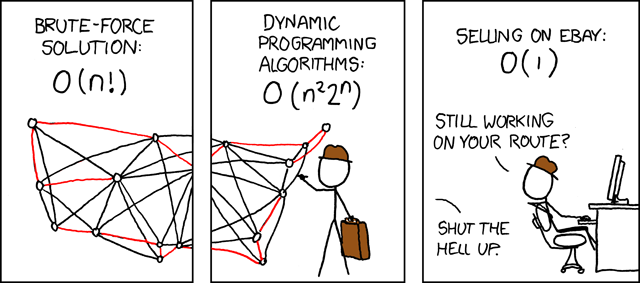
\includegraphics[width=\textwidth]{images/travelling_salesman_problem}
\end{frame}

\end{document}
